
%=========================================================================
% Start of
%=========================================================================
\preClass{Distance and Circles}

\begin{problem}
\item Expand each of the functions below by FOILing the
  expression. The first one is done as an example. Recall what it
  means to FOIL an expression.

  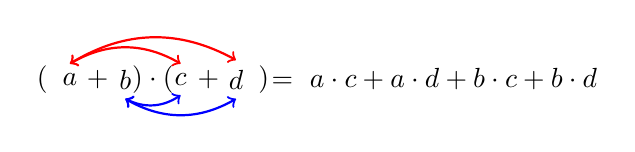
\begin{tikzpicture}[y=1em, x=1em,font=\sffamily]
    %% Draw the (a+b) part
    \node     at (0,0) {$($};
    \node (a) at (1,0) {$a$};
    \node     at (2,0) {$+$};
    \node (b) at (3,0) {$b$};
    \node     at (4,0) {$)\cdot($};

    %% Draw the *(c+d) part
    \node (c) at (5,0) {$c$};
    \node     at (6,0) {$+$};
    \node (d) at (7,0) {$d$};
    \node     at (8,0) {$)$};

    %% Draw the right hand side of the equation
    \node     at (14,0) {$~=~a\cdot c + a\cdot d + b\cdot c + b\cdot d$};

    %% Now make the pretty lines between the parts to FOIL
    \path[red,<->,thick] (a.north) edge[bend left] node {} (c.north);
    \path[red,<->,thick] (a.north) edge[bend left] node {} (d.north);

    \path[blue,<->,thick] (b.south) edge[bend right] node {} (c.south);
    \path[blue,<->,thick] (b.south) edge[bend right] node {} (d.south);

  \end{tikzpicture}

  \begin{subproblem}
  \item ${\displaystyle (x-3)^2}$
    \begin{eqnarray*}
      (x-3)^2 & = & (x-3)\cdot(x-3), \\
              & = & x\cdot x - 3\cdot x - 3\cdot x + (-3)\cdot(-3), \\
              & = & x^2 - 3x - 3x + 9, \\
              & = & x^2 - 6x + 9.
    \end{eqnarray*}
  \item ${\displaystyle (x+4)^2}$
    \vfill
  \item ${\displaystyle (y-5)^2}$
    \vfill
  \item ${\displaystyle (y+a)^2}$ where $a$ is a constant.
    \vfill
  \end{subproblem}
\item if $(x-a)^2=x^2+10x+25$ what is the value of $a$?
  \vfill
\end{problem}


\actTitle{Graphs of Equations}
\begin{problem}

\item Sketch the set of all points that are a distance of two from the
  point $Q(1,-3)$. What kind of figure do the points represent?

  \begin{tikzpicture}[y=1cm, x=1cm,font=\sffamily]
      % bounds
      \def\lowX{-5.5}
      \pgfmathtruncatemacro\startX{round(0.5+\lowX)}
      \pgfmathsetmacro\nextXValue{int(\startX+1)}
      \def\highX{5.5}
      \def\lowY{-5.5}
      \def\highY{5.5}
      \pgfmathsetmacro\nextYValue{int(\lowY+1)}
      % ticks
      \draw[step = 1, gray, very thin,dashed,opacity=0.85] (\lowX, \lowY) grid ( \highX,\highY);
   	% axis
  	\draw[thick,->] (\lowX,0) -- coordinate (x axis mid) (\highX,0) node[anchor = north west] {$x$};
      \draw[thick,->] (0,\lowY) -- coordinate (y axis mid) (0,\highY) node[anchor = south east] {$y$};
      \foreach \y in {-5,-4,...,-1,1,2,...,\highY} {
        \draw (1pt, \y) -- (-1pt, \y) node[yshift=-6,xshift=-1,anchor=east] {$\y$};
      }
      \foreach \x in {-5,-4,...,-1,1,2,...,\highX} {
        \draw (\x,1pt) -- (\x,-1pt) node[yshift=-5,xshift=-1,anchor=east] {$\x$};
      }
    \end{tikzpicture}


\item Suppose a point, $P(x,y)$ is a distance of $R$ units from the
  point $C(x_0,y_0)$.
  \sideNote{The values, $x_0$ and $y_0$, are constants. The notation
    is awkward, but this is a convention that we have to adapt to.}
  \begin{subproblem}
  \item Use the distance formula to express the distance relationship
    between $P$ and $C$.
    \vfill
  \item Square both sides of the previous equation.
    \vfill
  \end{subproblem}


\clearpage

\item Make a sketch of the circle with a radius of two centered at the
  point $P(-2,3)$. Determine a formula for the circle.

  \begin{tikzpicture}[y=1cm, x=1cm,font=\sffamily]
    % bounds
    \def\lowX{-5.5}
    \pgfmathtruncatemacro\startX{round(0.5+\lowX)}
    \pgfmathsetmacro\nextXValue{int(\startX+1)}
    \def\highX{5.5}
    \def\lowY{-5.5}
    \def\highY{5.5}
    \pgfmathsetmacro\nextYValue{int(\lowY+1)}
    % ticks
    \draw[step = 1, gray, very thin,dashed,opacity=0.85] (\lowX, \lowY) grid ( \highX,\highY);
 	% axis
	\draw[thick,->] (\lowX,0) -- coordinate (x axis mid) (\highX,0) node[anchor = north west] {$x$};
    \draw[thick,->] (0,\lowY) -- coordinate (y axis mid) (0,\highY) node[anchor = south east] {$y$};
    \foreach \y in {-5,-4,...,-1,1,2,...,\highY} {
      \draw (1pt, \y) -- (-1pt, \y) node[yshift=-6,xshift=-1,anchor=east] {$\y$};
    }
    \foreach \x in {-5,-4,...,-1,1,2,...,\highX} {
      \draw (\x,1pt) -- (\x,-1pt) node[yshift=-5,xshift=-1,anchor=east] {$\x$};
    }
  \end{tikzpicture}

  \clearpage

\item Sketch a graph of the relationship given by
  \begin{eqnarray*}
    x^2 + 2x + y^2 - 8y & = & 8.
  \end{eqnarray*}
  Determine the center and the radius of the circle.  Make a sketch of
  the circle. (Include the axes and label the axes.)  

  \vfill

  \clearpage

\item Windows are constructed, and their width is proportional to
  their height. One window is measured, and its width is 100cm, and its
  height is 200cm. 

  \begin{subproblem}

  \item Another window has a width of 75cm. What is its height?

    \vfill

  \item Make a sketch of the relationship of the height of a window
    given its width. First, express the relationship as a mathematical
    formula. Second, sketch the graph of the relationship. Briefly
    discuss the relationship. How does the height change as the width
    changes?  \sideNote{Annotate your plot and label your axes!}

    \vfill
    
  \end{subproblem}

  \clearpage

\item The surface area of a sparrow's wing is proportional to the
  square of the length of its wing. A sparrow is measured, and it has
  a wing length of 9cm and an area of 45cm\textsuperscript{2}. 

  \begin{subproblem}

  \item Another sparrow is measured, and the length of its wing is
    8cm. What is the area of its wing?

    \vfill

  \item Make a sketch of the relationship of the area of a sparrow's
    wing given the length. Briefly discuss the relationship. How does
    the area change as the length changes?  \sideNote{Annotate your
      plot and label your axes!}

    \vfill

  \end{subproblem}

  \vfill



\end{problem}

\postClass

\begin{problem}
\item Briefly state two ideas from today's class.
  \begin{itemize}
  \item
  \item
  \end{itemize}
\item A square is circumscribed within a circle of radius $R$ so it
  just touches the circle on each of the four corners of the square.

  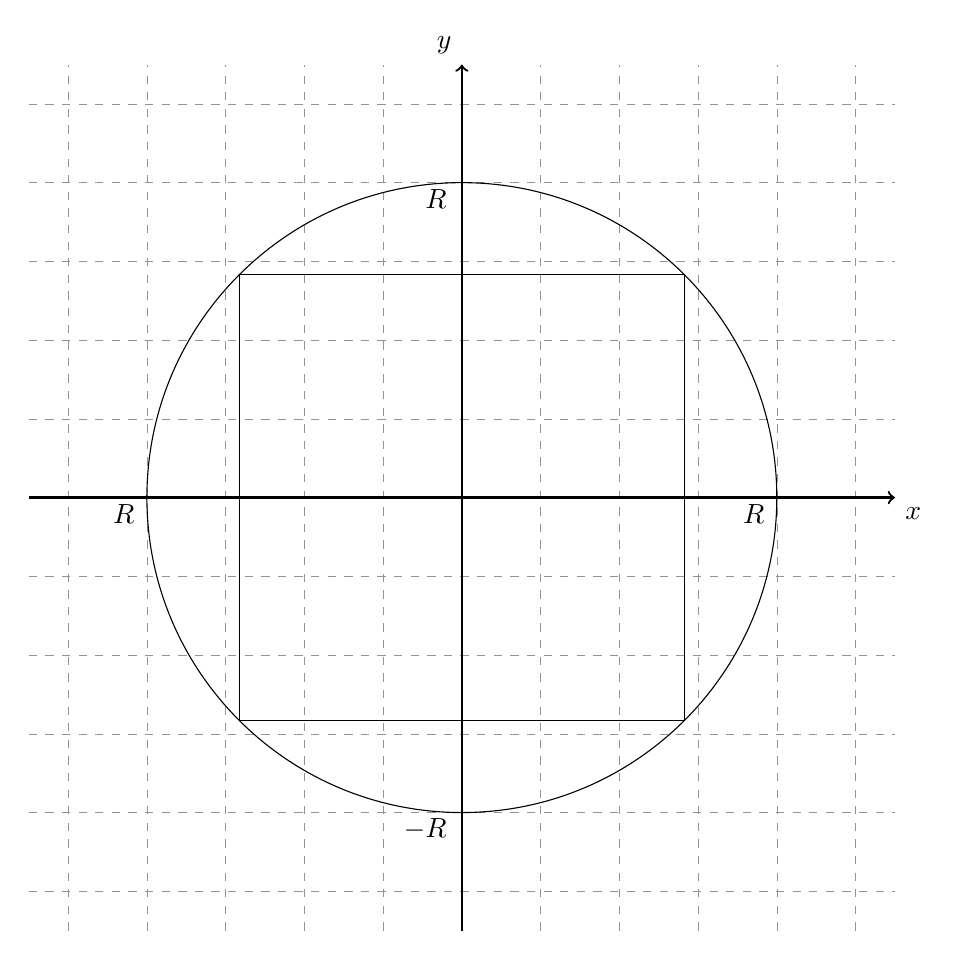
\begin{tikzpicture}[y=1cm, x=1cm,font=\sffamily]
    % bounds
    \def\lowX{-5.5}
    \pgfmathtruncatemacro\startX{round(0.5+\lowX)}
    \pgfmathsetmacro\nextXValue{int(\startX+1)}
    \def\highX{5.5}
    \def\lowY{-5.5}
    \def\highY{5.5}
    \pgfmathsetmacro\nextYValue{int(\lowY+1)}
    % ticks
    \draw[step = 1, gray, very thin,dashed,opacity=0.85] (\lowX, \lowY) grid ( \highX,\highY);
 	% axis
	\draw[thick,->] (\lowX,0) -- coordinate (x axis mid) (\highX,0) node[anchor = north west] {$x$};
    \draw[thick,->] (0,\lowY) -- coordinate (y axis mid) (0,\highY) node[anchor = south east] {$y$};

    \draw[black] (0:4) arc (0:360:4);
    \draw[black] (45:4) -- (135:4) -- (225:4) -- (315:4) -- (45:4);
    %\draw[black] (0:0) arc (0:30:0.2) node[midway,anchor=west] {$\theta$};

    \draw (1pt,  4) -- (-1pt,  4) node[yshift=-6,xshift=-1,anchor=east] {$R$};
    \draw (1pt, -4) -- (-1pt, -4) node[yshift=-6,xshift=-1,anchor=east] {$-R$};

    \draw ( 4,1pt) -- ( 4,-1pt) node[yshift=-5,xshift=-1,anchor=east] {$R$};
    \draw (-4,1pt) -- (-4,-1pt) node[yshift=-5,xshift=-1,anchor=east] {$R$};

  \end{tikzpicture}

  \begin{subproblem}
    \item Sketch the radius of the circle at one of the points where the square touches the circle.
    \item Find a convenient right triangle in the new diagram using
      the radius that you drew, and use the triangle to determine the
      length of one of the sides of the square. (You may have to
      double the length of the triangle to get the length of the
      side.)
    \item Determine the area of the square.
  \end{subproblem}

\item A triangle with three equal sides is circumscribed within a
  circle of radius $R$ so it just touches the circle on each of the
  three corners of the triangle.

  \begin{subproblem}
  \item Make a sketch of the situation. (Label your axes and label the
    length of the sides of the triangle.)
  \item Sketch the radius of the circle at one of the points where the
    triangle touches the circle.
  \item Find a convenient right triangle in the new diagram, and use
    the triangle to determine the length of one of the sides of the
    triangle. (You may have to double the length of the triangle to
    get the length of the side.)
  \end{subproblem}


\end{problem}



%%% Local Variables:
%%% mode: latex
%%% TeX-master: "functions"
%%% End:
